% flashcards-title: Array of counters with one row and one column marked
% flashcards-desc: Counters arranged in a rectangular array of 3 rows and 5 columns. An arrow above the top row is labeled row, and an arrow beside the left column is labeled column. No totals or statements are shown.
\documentclass[tikz]{standalone}
\usetikzlibrary{arrows.meta,patterns}

\definecolor{qraNavy}{HTML}{17324D}
\definecolor{qraBlue}{HTML}{2B6CB0}
\definecolor{qraGold}{HTML}{B7791F}
\definecolor{qraPale}{HTML}{EAF2F8}
\definecolor{qraGray}{HTML}{5C6773}

\tikzset{
  qra axis/.style={draw=qraNavy, line width=1.2pt},
  qra tick/.style={draw=qraNavy, line width=1pt},
  qra guide/.style={draw=qraGray, densely dashed, line width=0.8pt},
  qra counter/.style={circle, draw=qraNavy, fill=qraPale, line width=0.9pt, minimum size=7mm, inner sep=0pt},
  qra label/.style={font=\sffamily\bfseries, text=qraNavy},
  qra small label/.style={font=\sffamily, text=qraNavy},
}

\begin{document}
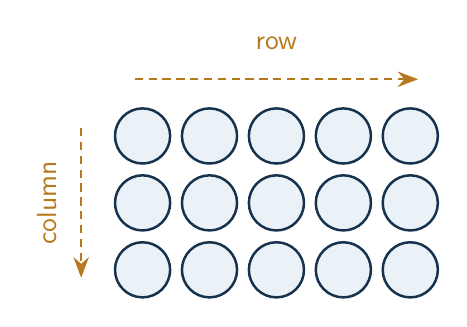
\begin{tikzpicture}
  % Array: 3 rows (j) x 5 columns (i)
  \foreach \i in {0,...,4} {
    \foreach \j in {0,1,2} {
      \node[qra counter] at (\i*0.85, -\j*0.85) {};
    }
  }

  % Row arrow above the top row
  \draw[qra guide, draw=qraGold, -{Stealth[length=2.6mm]}]
    (-0.1,0.72) -- (3.5,0.72);
  \node[qra small label, text=qraGold] at (1.7,1.18) {row};

  % Column arrow beside the left column
  \draw[qra guide, draw=qraGold, -{Stealth[length=2.6mm]}]
    (-0.78,0.1) -- (-0.78,-1.8);
  \node[qra small label, text=qraGold, rotate=90] at (-1.22,-0.85) {column};
\end{tikzpicture}
\end{document}
